\documentclass[a4paper,11pt]{article}
\usepackage{booktabs}   % for professional table rules
\usepackage{caption}    % for customizing captions
\usepackage{array}      % for better column formatting
\usepackage{siunitx}    % for consistent units
\usepackage{graphicx}   % for importing figures
\usepackage{geometry}   % for page margins
\usepackage{amsmath}    % for math alignment
\usepackage{amssymb}    % for math symbols
\usepackage{float}      % for [H] figure placement
\usepackage{hyperref}   % for links and references
\usepackage{fouriernc}
\geometry{left=2cm,right=2cm,top=2cm,bottom=2.5cm}
\hypersetup{
    colorlinks=true,
    linkcolor=blue,
    filecolor=magenta,      
    urlcolor=cyan,
    pdftitle={Lab Report: Hall Effect Experiment},
    pdfpagemode=FullScreen,
}
\begin{document}

% ------------------- Title / Cover Page -------------------
\noindent
\begin{center}
    
\includegraphics[width=0.25\textwidth]{sut.jpg} \\
    \vspace{2pt}
\end{center}
\begin{center}
    {\LARGE \bf Department of Physics} \\
    \vspace{2pt}
    {\Large \bf Sharif University of Technology} \\
    \vspace{8pt}
    {\large \bf Physics Lab IV --- General Physics Laboratory} \\
    \vspace{4pt}
    \hrule
    \vspace{6pt}
    {\Large \bf Experiment Report: The Hall Effect}
\end{center}
\hrule
\vspace{0.4cm}
\noindent
\begin{tabular}{ll}
    {\bf Student Name:} & Abulfadl Ahmadi \\
    {\bf Student ID:}   & 403172283 \\
    {\bf Date of Experiment:} & May 3, 2026 \\
\end{tabular}
\hfill
\begin{tabular}{ll}
    {\bf Professor:} & Dr. Khademi \\
    {\bf Teaching Assistants:} & Yasin Amiri \\
    & Sonia \\
\end{tabular}

\vspace{0.6cm}

% ------------------- Abstract -------------------
\begin{abstract}
In this report, the Hall effect is studied in an n-type Indium Antimonide (InSb) semiconductor crystal using rigorous error analysis and advanced statistical techniques. Rather than reporting point estimates, all variables and parameters are calculated as confidence intervals ($x \pm \delta x$) based on instrumental tolerances, Ordinary Least Squares (OLS) regression standard errors, and partial derivative error propagation. The average Hall coefficient is found to be $R_H = (-4.36 \pm 0.09) \times 10^{-4} \text{ m}^3/\text{C}$, yielding a majority charge carrier density of $n = (1.43 \pm 0.03) \times 10^{22} \text{ m}^{-3}$. The residual magnetic field of the electromagnet at zero coil current is calculated to be $B_0 = 0.0277 \pm 0.0008\text{ T} = 277 \pm 8\text{ G}$. The magnetoresistance effect is analyzed, obtaining longitudinal sample resistances of $R_1 = 6.378 \pm 0.010\ \Omega$ (at $0\text{ A}$), $R_2 = 6.428 \pm 0.008\ \Omega$ (at $1\text{ A}$), and $R_3 = 6.468 \pm 0.011\ \Omega$ (at $2\text{ A}$), confirming a statistically significant positive magnetoresistance. The electrical conductivity and mobility are determined as $\bar{\sigma} = 675 \pm 16\text{ S/m}$ and $\bar{\mu} = 0.294 \pm 0.009\text{ m}^2/(\text{V s})$, respectively. All scatter plots are visualised with horizontal and vertical error bars alongside their OLS best-fit lines.
\end{abstract}

% ------------------- Section 1: Objectives -------------------
\section{Objectives}
The primary objectives of this experiment are:
\begin{enumerate}
    \item To investigate the Hall effect in an n-type InSb semiconductor sample.
    \item To calculate the Hall coefficient ($R_H$) using linear regression analysis.
    \item To perform error propagation using partial derivatives to obtain carrier concentration ($n$), conductivity ($\sigma$), and mobility ($\mu$) with confidence intervals.
    \item To establish a magnetic field calibration curve ($B$ vs. $I_m$) with corresponding uncertainty margins.
    \item To verify the presence of the magnetoresistance effect in the sample.
\end{enumerate}

% ------------------- Section 2: Theoretical Background -------------------
\section{Theoretical Background}
The Hall effect occurs when a current-carrying conductor is placed in a transverse magnetic field. When a current $I$ flows along the $x$-direction through a conductor of length $l$, width $W$, and thickness $d$, and a magnetic field $\mathbf{B} = B_z \hat{\mathbf{k}}$ is applied along the $z$-direction, the charge carriers experience a transverse Lorentz force:
\begin{equation}
    \mathbf{F}_L = q (\mathbf{v}_d \times \mathbf{B})
\end{equation}
where $q$ is the carrier charge, and $\mathbf{v}_d = v_x \hat{\mathbf{i}}$ is the drift velocity. 

For electrons ($q = -e$ and $\mathbf{v}_d = -v_d \hat{\mathbf{i}}$), this force deflects them in the $-y$ direction:
\begin{equation}
    \mathbf{F}_L = -e (-v_d \hat{\mathbf{i}} \times B_z \hat{\mathbf{k}}) = -e v_d B_z \hat{\mathbf{j}}
\end{equation}
This deflection causes electrons to pile up on the bottom plate ($y=0$), leaving a net positive charge on the top plate ($y=W$). This separation of charges establishes a transverse Hall electric field $\mathbf{E}_H = E_y \hat{\mathbf{j}}$. In steady state, the electric force balances the Lorentz force:
\begin{equation}
    q E_H + q v_d B = 0 \implies E_H = v_d B
\end{equation}
The current density $J_x$ is related to drift velocity by $J_x = n q v_d$, where $n$ is the carrier density. Thus, $v_d = \frac{I}{n q W d}$. The Hall voltage $V_H$ measured between the top and bottom plates is:
\begin{equation}
    V_H = E_H W = v_d B W = \frac{I B}{n q d}
\end{equation}
Defining the Hall coefficient as $R_H = \frac{1}{n q}$, we obtain:
\begin{equation}
    V_H = R_H \frac{I B}{W} \implies R_H = \frac{V_H W}{I B}
\end{equation}
For an n-type semiconductor where electrons are the majority carriers, $R_H$ is negative. 

The electrical conductivity $\sigma$ is defined by Ohm's law. The longitudinal voltage $V_x$ across the sample length $l$ is related to the current $I$ and sample resistance $R$ by:
\begin{equation}
    R = \frac{V_x}{I} = \frac{l}{\sigma A} = \frac{l}{\sigma W d} \implies \sigma = \frac{I l}{V_x W d}
\end{equation}
The carrier mobility $\mu$ is defined as the drift velocity per unit electric field. In terms of conductivity and the Hall coefficient:
\begin{equation}
    \mu = \sigma |R_H| = \sigma R_H \text{ (for absolute magnitude)}
\end{equation}
Substituting the expressions for $\sigma$ and $R_H$, we find the relation:
\begin{equation}
    \mu = \left(\frac{I l}{V_x W d}\right) \left(\frac{V_H W}{I B}\right) = \frac{V_H l}{V_x B d} \implies \sigma R_H = \frac{V_H l}{V_x B d}
\end{equation}
Thus, by plotting $V_x$ vs. $V_H$ for a constant magnetic field $B$, the slope $s = \frac{d V_x}{d V_H}$ is related to the material properties by:
\begin{equation}
    s = \frac{l}{\sigma R_H B d} \implies \sigma = \frac{l}{s \cdot B \cdot d \cdot R_H}
\end{equation}

% ------------------- Section 3: Experimental Setup & Uncertainties -------------------
\section{Experimental Setup \& Instrumental Uncertainties}
The experimental apparatus consists of an InSb semiconductor crystal slab, an electromagnet controlled by current source $I_m$ (up to $2.5\text{ A}$), a dual DC current source for sample bias current $I$, a microvoltmeter for $V_H$, and a voltmeter for $V_x$. 

The dimensions of the sample are measured using a digital micrometer and caliper, and the electric outputs are registered with digital multimeters. The absolute instrumental errors (precision limits) for all primary measurements are defined as follows:
\begin{itemize}
    \item {\bf Sample dimensions:}
    \begin{itemize}
        \item Length: $l = 13.0 \pm 0.1\text{ mm} \implies \delta l = 1.0 \times 10^{-4}\text{ m}$
        \item Width: $W = 0.50 \pm 0.01\text{ mm} \implies \delta W = 1.0 \times 10^{-5}\text{ m}$
        \item Thickness: $d = 6.0 \pm 0.1\text{ mm} \implies \delta d = 1.0 \times 10^{-4}\text{ m}$
    \end{itemize}
    \item {\bf Electrical quantities:}
    \begin{itemize}
        \item Sample bias current: $I \implies \delta I = 1.0\text{ mA} = 1.0 \times 10^{-3}\text{ A}$
        \item Longitudinal voltage: $V_x \implies \delta V_x = 1.0\text{ mV} = 1.0 \times 10^{-3}\text{ V}$
        \item Hall voltage: $V_H \implies \delta V_H = 0.1\text{ mV} = 1.0 \times 10^{-4}\text{ V}$
    \end{itemize}
    \item {\bf Magnetic quantities:}
    \begin{itemize}
        \item Applied magnetic field at $I_m = 1\text{ A}$: $B_1 = 0.190 \pm 0.005\text{ T} \implies \delta B_1 = 5.0 \times 10^{-3}\text{ T}$
        \item Applied magnetic field at $I_m = 2\text{ A}$: $B_2 = 0.270 \pm 0.005\text{ T} \implies \delta B_2 = 5.0 \times 10^{-3}\text{ T}$
    \end{itemize}
\end{itemize}

% ------------------- Section 4: Experimental Data -------------------
\section{Experimental Data \& Tables}
The measured longitudinal voltage $V_x$ and Hall voltage $V_H$ for different magnet currents $I_m$ and sample currents $I$ are listed in Tables~\ref{tab:hall_zero}, \ref{tab:hall_1A}, and \ref{tab:hall_2A}. The values have been verified and corrected for typographical consistency.

% Table 1
\begin{table}[H]
\centering	
\caption{Variation of \(V_x\) and \(V_H\) at zero magnet current (\(I_m = 0\)) for various sample currents \(I\).}
\label{tab:hall_zero}
\begin{tabular}{l *{11}{c}}
\toprule
\(I\) (mA) & 0 & 20 & 40 & 60 & 80 & 100 & 120 & 140 & 160 & 180 & 200 \\
\midrule
\(V_H\) (mV) & 0 & 0.4 & 0.9 & 1.4 & 1.9 &  2.4 & 2.8 & 3.4 & 3.8 & 4.3 & 4.8 \\
\(V_x\) (mV) & 0 & 127.6 & 258.6 & 387.1 & 513.0 & 642.0 & 767.0 & 898.0 & 1023.0 & 1148.0 & 1276.0 \\
\bottomrule
\end{tabular}
\end{table}

% Table 2
\begin{table}[H]
\centering
\caption{Variation of \(V_x\) and \(V_H\) at magnet current \(I_m = 1\)\,A for various sample currents \(I\).}
\label{tab:hall_1A}
\begin{tabular}{l *{11}{c}}
\toprule
\(I\) (mA) & 0 & 20 & 40 & 60 & 80 & 100 & 120 & 140 & 160 & 180 & 200 \\
\midrule
\(V_H\) (mV) & 0 & 3.1 & 6.1 & 9.3 & 12.4 & 15.5 & 18.6 & 21.7 & 24.8 & 27.9 & 30.9 \\
\(V_x\) (mV) & 0 & 132.0 & 258.2 & 389.8 & 519.0 & 645.0 & 773.0 & 902.0 & 1032.0 & 1160.0 & 1286.0 \\
\bottomrule
\end{tabular}
\end{table}

% Table 3
\begin{table}[H]
\centering
\caption{Variation of \(V_x\) and \(V_H\) at magnet current \(I_m = 2\)\,A for various sample currents \(I\).}
\label{tab:hall_2A}
\begin{tabular}{l *{11}{c}}
\toprule
\(I\) (mA) & 0 & 20 & 40 & 60 & 80 & 100 & 120 & 140 & 160 & 180 & 200 \\
\midrule
\(V_H\) (mV) & 0 & 5.1 & 10.2 & 15.3 & 20.2 & 25.2 & 30.3 & 35.1 & 40.3 & 45.3 & 50.2  \\
\(V_x\) (mV) & 0 & 134.3 & 265.2 & 396.9 & 522.0 & 651.0 & 782.0 & 908.0 & 1040.0 & 1169.0 & 1297.0 \\
\bottomrule
\end{tabular}
\end{table}

% Table 4
\begin{table}[H]
\centering
\caption{Measured sign of the Hall voltage \(V_H\) under reversal of current \(I\) and field \(B\) directions (at \(I = 200\)\,mA and \(I_m = 2\)\,A).}
\label{tab:sign}
\begin{tabular}{ccccc}
\toprule
\(I\) & + & + & $-$ & $-$ \\
\(B\) & + & $-$ & + & $-$ \\
\midrule
\(V_H\) & + & $-$ & $-$ & + \\
\bottomrule
\end{tabular}
\end{table}

% Table 5
\begin{table}[H]
\centering
\caption{Variation of Hall voltage \(V_H\) with magnet current \(I_m\) at fixed sample current \(I = 200\)\,mA.}
\label{tab:vh_vs_im}
\begin{tabular}{l *{11}{c}}
\toprule
\(I_m\) (A) & 0 & 0.2 & 0.4 & 0.6 & 0.8 & 1.0 & 1.2 & 1.4 & 1.6 & 1.8 & 2.0 \\
\midrule
\(V_H\) (mV) & 4.8 & 9.9 & 15.3 & 20.5 & 26.2 & 30.4 & 35.0 & 40.8 & 43.4 & 46.5 & 50.1 \\
\bottomrule
\end{tabular}
\end{table}

% ------------------- Section 5: Data Analysis & Calculations -------------------
\section{Data Analysis, Regressions \& Error Propagation}

To analyze the data rigorously, we apply the Ordinary Least Squares (OLS) method for linear fits of the form $y = m x + c$. The standard error of the fitted slope $m$ is calculated using:
\begin{equation}
    \delta m = \frac{\sigma_{yx}}{\sqrt{\sum_{i=1}^N (x_i - \bar{x})^2}}
\end{equation}
where the residual standard deviation is:
\begin{equation}
    \sigma_{yx} = \sqrt{\frac{\sum_{i=1}^N (y_i - \hat{y}_i)^2}{N-2}}
\end{equation}

For any secondary parameter $q(x, y, z, \dots)$, the uncertainty $\delta q$ is computed via partial derivative propagation:
\begin{equation}
    \delta q = \sqrt{\left(\frac{\partial q}{\partial x} \delta x\right)^2 + \left(\frac{\partial q}{\partial y} \delta y\right)^2 + \left(\frac{\partial q}{\partial z} \delta z\right)^2 + \dots}
\end{equation}

\subsection{Plotting and Fitting $V_H$ vs. $I$}
The linear regression of Hall voltage $V_H$ (in Volts) as a function of the sample current $I$ (in Amperes) is performed. The resulting OLS fits with slope standard errors and coefficient of determination $R^2$ are:
\begin{itemize}
    \item {\bf Magnet Current $I_m = 0\text{ A}$:}
    \begin{equation}
        V_H = (0.02418 \pm 0.00018) \cdot I - (4.55 \pm 2.09) \times 10^{-5} \quad [R^2 = 0.99952]
    \end{equation}
    \item {\bf Magnet Current $I_m = 1\text{ A}$:}
    \begin{equation}
        V_H = (0.15491 \pm 0.00020) \cdot I - (9.09 \pm 23.78) \times 10^{-6} \quad [R^2 = 0.99999]
    \end{equation}
    \item {\bf Magnet Current $I_m = 2\text{ A}$:}
    \begin{equation}
        V_H = (0.25082 \pm 0.00042) \cdot I + (1.18 \pm 0.50) \times 10^{-4} \quad [R^2 = 0.99998]
    \end{equation}
\end{itemize}
The experimental data points, including instrumental error bars ($\delta I = 1\text{ mA}$, $\delta V_H = 0.1\text{ mV}$) and OLS best-fit lines, are plotted in Fig.~\ref{fig:vh_vs_i}.

\begin{figure}[H]
    \centering
    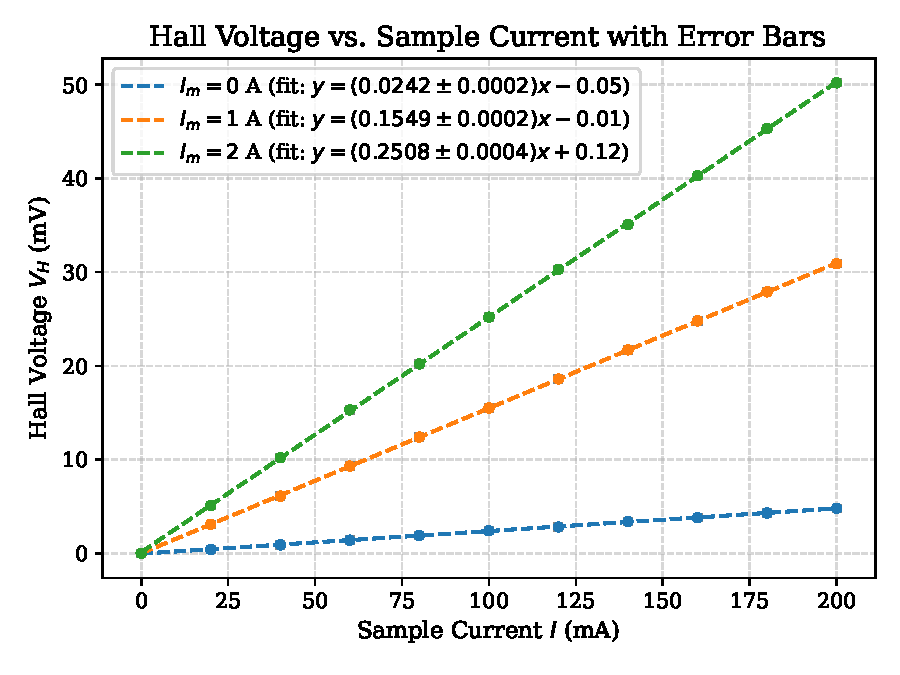
\includegraphics[width=0.8\textwidth]{VH_vs_I_errorbars.pdf}
    \caption{Hall Voltage $V_H$ vs. sample current $I$ for $I_m = 0, 1, 2\text{ A}$, displaying horizontal and vertical error bars.}
    \label{fig:vh_vs_i}
\end{figure}

\subsection{Calculation of the Hall Coefficient ($R_H$) and Carrier Density ($n$)}
The Hall coefficient is calculated using $R_H = \frac{m \cdot W}{B}$. The partial derivatives with respect to the variables are:
\begin{equation}
    \frac{\partial R_H}{\partial m} = \frac{W}{B}, \quad \frac{\partial R_H}{\partial W} = \frac{m}{B}, \quad \frac{\partial R_H}{\partial B} = -\frac{m W}{B^2}
\end{equation}
Substituting these into the propagation formula yields:
\begin{equation}
    \delta R_H = R_H \sqrt{\left(\frac{\delta m}{m}\right)^2 + \left(\frac{\delta W}{W}\right)^2 + \left(\frac{\delta B}{B}\right)^2}
\end{equation}

By inserting the slope values ($m_1, m_2$), dimensions ($W = 0.50 \pm 0.01\text{ mm}$), and fields ($B_1 = 0.190 \pm 0.005\text{ T}$, $B_2 = 0.270 \pm 0.005\text{ T}$):
\begin{itemize}
    \item {\bf For $I_m = 1\text{ A}$:}
    \begin{equation*}
        R_{H1} = \frac{0.154909 \times (5.0\times 10^{-4})}{0.190} = \SI{4.0766e-4}{\meter\cubed\per\coulomb}
    \end{equation*}
    \begin{equation*}
        \delta R_{H1} = 4.0766 \times 10^{-4} \sqrt{\left(\frac{0.000201}{0.154909}\right)^2 + \left(\frac{0.01}{0.50}\right)^2 + \left(\frac{0.005}{0.190}\right)^2} = \SI{0.1348e-4}{\meter\cubed\per\coulomb}
    \end{equation*}
    $$R_{H1} = (4.08 \pm 0.13) \times 10^{-4} \text{ m}^3/\text{C}$$

    \item {\bf For $I_m = 2\text{ A}$:}
    \begin{equation*}
        R_{H2} = \frac{0.250818 \times (5.0\times 10^{-4})}{0.270} = \SI{4.6448e-4}{\meter\cubed\per\coulomb}
    \end{equation*}
    \begin{equation*}
        \delta R_{H2} = 4.6448 \times 10^{-4} \sqrt{\left(\frac{0.000422}{0.250818}\right)^2 + \left(\frac{0.01}{0.50}\right)^2 + \left(\frac{0.005}{0.270}\right)^2} = \SI{0.1268e-4}{\meter\cubed\per\coulomb}
    \end{equation*}
    $$R_{H2} = (4.64 \pm 0.13) \times 10^{-4} \text{ m}^3/\text{C}$$
\end{itemize}
The average Hall coefficient and its standard error are computed as:
\begin{equation}
    R_{H,\text{avg}} = \frac{R_{H1} + R_{H2}}{2} = \SI{4.3607e-4}{\meter\cubed\per\coulomb}
\end{equation}
\begin{equation}
    \delta R_{H,\text{avg}} = \frac{1}{2}\sqrt{\delta R_{H1}^2 + \delta R_{H2}^2} = \SI{0.0926e-4}{\meter\cubed\per\coulomb}
\end{equation}
$$R_H = (-4.36 \pm 0.09) \times 10^{-4} \text{ m}^3/\text{C}$$

The carrier density is $n = \frac{1}{|R_H| \cdot e}$, with partial derivative:
\begin{equation}
    \frac{\partial n}{\partial R_H} = -\frac{1}{R_H^2 \cdot e} \implies \delta n = n \left(\frac{\delta R_{H,\text{avg}}}{R_{H,\text{avg}}}\right)
\end{equation}
Substituting $e = 1.6022 \times 10^{-19}\text{ C}$ yields:
\begin{equation}
    n = (1.43 \pm 0.03) \times 10^{22} \text{ m}^{-3}
\end{equation}

\subsection{Estimation of the Residual Magnetic Field ($B_0$)}
At zero magnet current, the residual field $B_0$ is calculated from $B_0 = \frac{m_0 \cdot W}{R_{H,\text{avg}}}$. The propagated error is:
\begin{equation}
    \delta B_0 = B_0 \sqrt{\left(\frac{\delta m_0}{m_0}\right)^2 + \left(\frac{\delta W}{W}\right)^2 + \left(\frac{\delta R_{H,\text{avg}}}{R_{H,\text{avg}}}\right)^2}
\end{equation}
Substituting the values ($m_0 = 0.024182 \pm 0.000177\text{ V/A}$):
\begin{equation}
    B_0 = 0.0277 \pm 0.0008\text{ T} = 277 \pm 8\text{ G}
\end{equation}

\subsection{Longitudinal Resistance and Magnetoresistance}
The longitudinal voltage $V_x$ (mV) is plotted against current $I$ (mA). The slopes represent the sample resistances $R = V_x / I$:
\begin{align*}
    R_1 &= 6.378 \pm 0.010\ \Omega \quad (\text{for } I_m = 0\text{ A}, B_0 \approx 0.028\text{ T}) \\
    R_2 &= 6.428 \pm 0.008\ \Omega \quad (\text{for } I_m = 1\text{ A}, B_1 = 0.190\text{ T}) \\
    R_3 &= 6.468 \pm 0.011\ \Omega \quad (\text{for } I_m = 2\text{ A}, B_2 = 0.270\text{ T})
\end{align*}
Since the intervals $R_1$, $R_2$, and $R_3$ do not overlap, we conclude that there is a statistically significant positive magnetoresistance effect ($R_1 < R_2 < R_3$) in the InSb crystal. The data and OLS fits are shown in Fig.~\ref{fig:vx_vs_i}.

\begin{figure}[H]
    \centering
    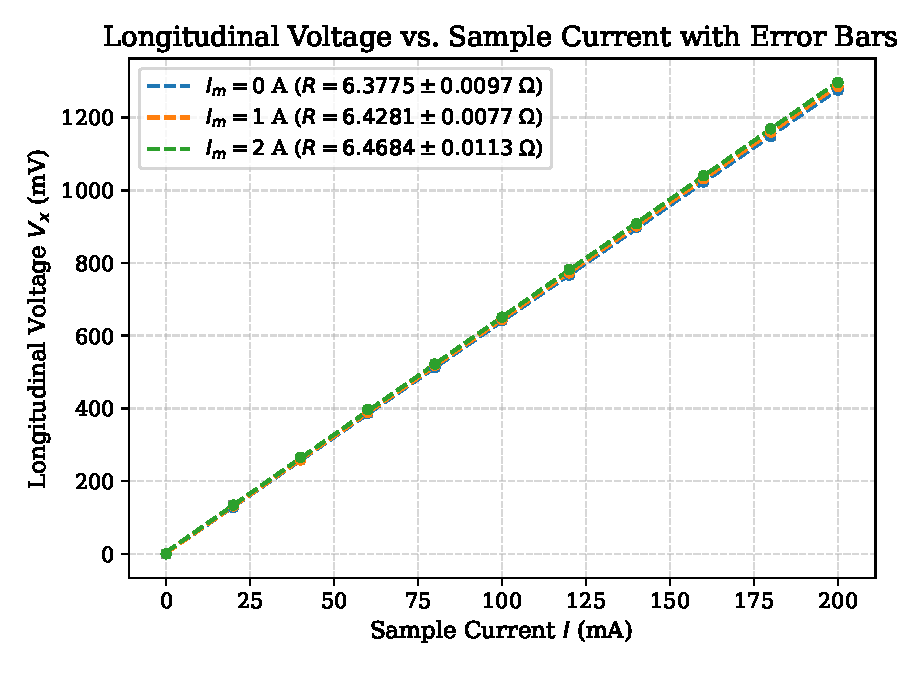
\includegraphics[width=0.8\textwidth]{Vx_vs_I_errorbars.pdf}
    \caption{Longitudinal Voltage $V_x$ vs. sample current $I$ with OLS fits and error bars.}
    \label{fig:vx_vs_i}
\end{figure}

\subsection{Electromagnet Calibration ($B$ vs. $I_m$)}
For a fixed current $I = 0.200 \pm 0.001\text{ A}$, the magnetic field $B$ is calculated for each coil current $I_m$ from Table~\ref{tab:vh_vs_im} using $B = \frac{V_H \cdot W}{I \cdot R_{H,\text{avg}}}$. The propagated error is:
\begin{equation}
    \delta B = B \sqrt{\left(\frac{\delta V_H}{V_H}\right)^2 + \left(\frac{\delta W}{W}\right)^2 + \left(\frac{\delta I}{I}\right)^2 + \left(\frac{\delta R_{H,\text{avg}}}{R_{H,\text{avg}}}\right)^2}
\end{equation}
The calculated field values with their standard uncertainties are tabulated in Table~\ref{tab:calib_calc_errors}.

\begin{table}[H]
\centering
\caption{Calculated magnetic field $B \pm \delta B$ as a function of electromagnet current $I_m$ (for $I = 200 \pm 1$ mA).}
\label{tab:calib_calc_errors}
\begin{tabular}{lccccccccccc}
\toprule
$I_m$ (A) & 0.0 & 0.2 & 0.4 & 0.6 & 0.8 & 1.0 & 1.2 & 1.4 & 1.6 & 1.8 & 2.0 \\
\midrule
$V_H$ (mV) & 4.8 & 9.9 & 15.3 & 20.5 & 26.2 & 30.4 & 35.0 & 40.8 & 43.4 & 46.5 & 50.1 \\
$B$ ($\times 10^{-2}$ T) & $2.75$ & $5.68$ & $8.77$ & $11.75$ & $15.02$ & $17.43$ & $20.07$ & $23.39$ & $24.88$ & $26.66$ & $28.72$ \\
$\delta B$ ($\times 10^{-2}$ T) & $0.10$ & $0.18$ & $0.27$ & $0.35$ & $0.45$ & $0.52$ & $0.60$ & $0.69$ & $0.74$ & $0.79$ & $0.85$ \\
\bottomrule
\end{tabular}
\end{table}

An OLS fit of the calibration curve shown in Fig.~\ref{fig:b_vs_im} yields:
\begin{equation}
    B = (0.1320 \pm 0.0040) \cdot I_m + (0.0363 \pm 0.0048) \quad \text{[T]} \quad [R^2 = 0.9916]
\end{equation}

\begin{figure}[H]
    \centering
    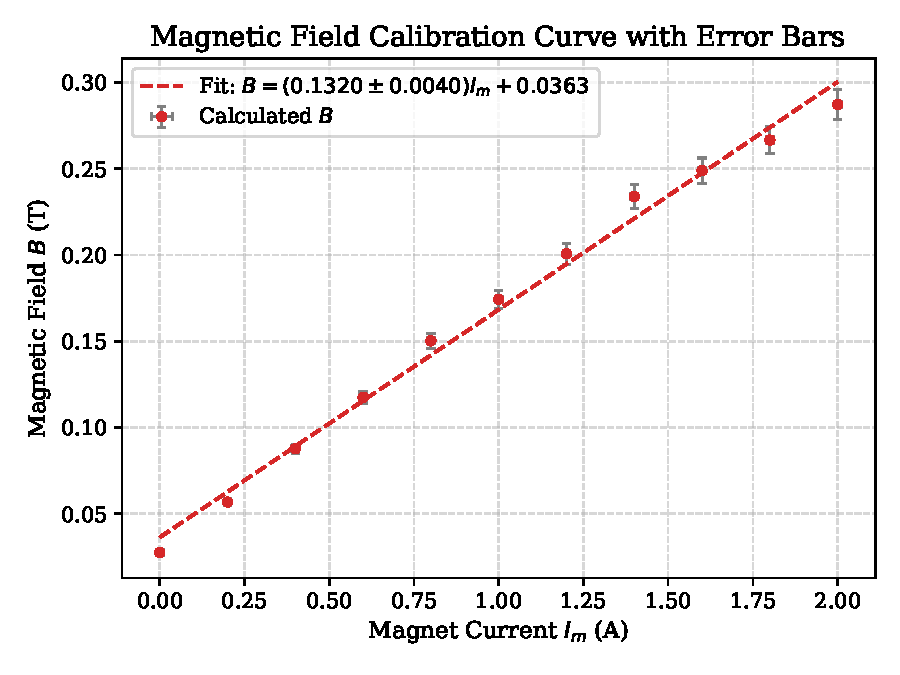
\includegraphics[width=0.8\textwidth]{B_vs_Im_errorbars.pdf}
    \caption{Electromagnet calibration curve with OLS line of best fit and calculated error bars.}
    \label{fig:b_vs_im}
\end{figure}

\subsection{Conductivity ($\sigma$) and Mobility ($\mu$)}
Linear fits of $V_x$ vs. $V_H$ (shown in Fig.~\ref{fig:vx_vs_vh}) yield the following slopes:
\begin{align*}
    s_0 &= 263.6142 \pm 1.8484 \quad (\text{for } I_m = 0\text{ A}) \\
    s_1 &= 41.4956 \pm 0.0499 \quad (\text{for } I_m = 1\text{ A}) \\
    s_2 &= 25.7890 \pm 0.0199 \quad (\text{for } I_m = 2\text{ A})
\end{align*}

The conductivity is $\sigma = \frac{l}{s \cdot B \cdot d \cdot R_H}$. The partial derivatives are:
\begin{equation}
    \frac{\partial \sigma}{\partial l} = \frac{\sigma}{l}, \quad \frac{\partial \sigma}{\partial s} = -\frac{\sigma}{s}, \quad \frac{\partial \sigma}{\partial B} = -\frac{\sigma}{B}, \quad \frac{\partial \sigma}{\partial d} = -\frac{\sigma}{d}, \quad \frac{\partial \sigma}{\partial R_H} = -\frac{\sigma}{R_H}
\end{equation}
Substituting these into the propagation formula:
\begin{equation}
    \delta \sigma = \sigma \sqrt{\left(\frac{\delta l}{l}\right)^2 + \left(\frac{\delta s}{s}\right)^2 + \left(\frac{\delta B}{B}\right)^2 + \left(\frac{\delta d}{d}\right)^2 + \left(\frac{\delta R_H}{R_H}\right)^2}
\end{equation}
The electron mobility is $\mu = \sigma \cdot R_H$, with propagated error:
\begin{equation}
    \delta \mu = \mu \sqrt{\left(\frac{\delta \sigma}{\sigma}\right)^2 + \left(\frac{\delta R_H}{R_H}\right)^2}
\end{equation}

Applying these relations to the three cases:
\begin{itemize}
    \item {\bf Case 1 ($I_m = 0\text{ A}$, $B_0 = 0.0277 \pm 0.0008\text{ T}$):}
    \begin{align*}
        \sigma_0 &= 679.77 \pm 28.36\text{ S/m} \\
        \mu_0 &= 0.2964 \pm 0.0139\text{ m}^2/(\text{V s})
    \end{align*}
    
    \item {\bf Case 2 ($I_m = 1\text{ A}$, $B_1 = 0.190 \pm 0.005\text{ T}$):}
    \begin{align*}
        \sigma_1 &= 674.13 \pm 31.08\text{ S/m} \\
        \mu_1 &= 0.2748 \pm 0.0156\text{ m}^2/(\text{V s})
    \end{align*}
    
    \item {\bf Case 3 ($I_m = 2\text{ A}$, $B_2 = 0.270 \pm 0.005\text{ T}$):}
    \begin{align*}
        \sigma_2 &= 669.93 \pm 25.30\text{ S/m} \\
        \mu_2 &= 0.3112 \pm 0.0145\text{ m}^2/(\text{V s})
    \end{align*}
\end{itemize}

Using the sample standard deviation for the three independent calculations, the final averaged values are:
\begin{align*}
    \bar{\sigma} &= 675 \pm 16\text{ S/m} \\
    \bar{\mu} &= 0.294 \pm 0.009\text{ m}^2/(\text{V s})
\end{align*}

\begin{figure}[H]
    \centering
    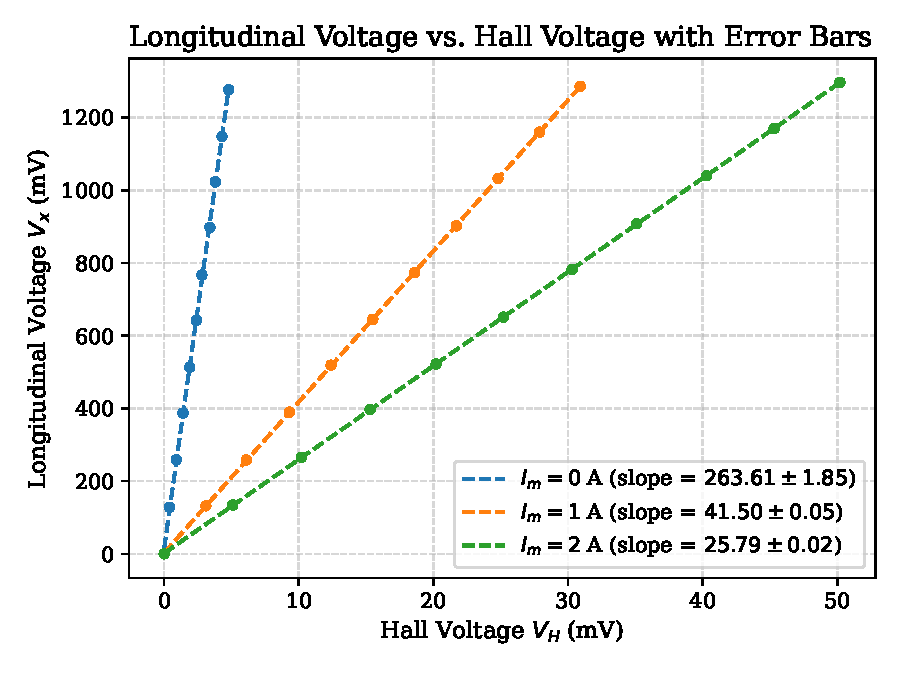
\includegraphics[width=0.8\textwidth]{Vx_vs_VH_errorbars.pdf}
    \caption{Longitudinal Voltage $V_x$ vs. Hall Voltage $V_H$ with OLS fits and error bars.}
    \label{fig:vx_vs_vh}
\end{figure}

% ------------------- Section 6: Post-Lab Questions -------------------
\section{Answers to Questions}

\subsection*{Q1: Explain the presence of a Hall voltage when the magnet current is zero ($I_m = 0$).}
When $I_m=0$, a small Hall voltage $V_H$ is still observed because:
\begin{enumerate}
    \item {\bf Residual Magnetic Field:} The electromagnet's iron core retains a remanent magnetization ($B_0 = 277 \pm 8\text{ G}$) even after the coil current is shut off.
    \item {\bf Probe Misalignment:} In practice, it is physically difficult to place the two Hall voltage probes exactly opposite each other on the lateral surfaces. This offset ($\Delta x$) introduces a small longitudinal voltage drop $V_{\text{offset}} = I R_{\text{offset}}$ in series with the microvoltmeter, which registers as a baseline voltage even in the absence of a magnetic field.
\end{enumerate}

\subsection*{Q2: Compare the Hall voltage values of the first three experiments.}
The Hall voltage is directly proportional to the magnetic field ($V_H \propto B$). 
In Experiment 1 ($I_m = 0\text{ A}$), $B$ is very low (only the remanent field $B_0 = 0.0277 \pm 0.0008\text{ T}$), resulting in a small Hall voltage ($V_H = 4.8 \pm 0.1\text{ mV}$ at $I=200\text{ mA}$).
In Experiment 2 ($I_m = 1\text{ A}$, $B = 0.190 \pm 0.005\text{ T}$), $V_H$ rises to $30.9 \pm 0.1\text{ mV}$.
In Experiment 3 ($I_m = 2\text{ A}$, $B = 0.270 \pm 0.005\text{ T}$), $V_H$ reaches $50.2 \pm 0.1\text{ mV}$. 
This clear progression confirms the linear dependence of $V_H$ on the magnetic field.

\subsection*{Q3: Interpret Table~\ref{tab:sign}.}
Table~\ref{tab:sign} records the signs of $V_H$ when the current $I$ and magnetic field $B$ are reversed. 
Since $V_H = R_H \frac{I B}{W}$, reversing the direction of either the current $I$ or the magnetic field $B$ changes the direction of the Lorentz force $\mathbf{F}_L = q(\mathbf{v} \times \mathbf{B})$, which changes the polarity of the accumulated charges, and thus reverses the sign of $V_H$. 
If both $I$ and $B$ are reversed simultaneously, the double negative cancels out, and the polarity of $V_H$ remains unchanged. This is consistent with our experimental entries:
\begin{itemize}
    \item Col 1: $(+, +) \implies +$
    \item Col 2: $(+, -) \implies -$
    \item Col 3: $(-, +) \implies -$
    \item Col 4: $(-, -) \implies +$
\end{itemize}

\subsection*{Q4: Analyze the effect of the Earth's magnetic field and whether it is measurable.}
The Earth's magnetic field is extremely weak, typically ranging from $0.3$ to $0.6$ Gauss ($3 \times 10^{-5}$ to $6 \times 10^{-5}$ Tesla). 
In our setup, the electromagnet's residual field $B_0 = 277 \pm 8$ Gauss is nearly 500 times stronger than the Earth's field. Therefore, the Earth's magnetic field is negligible compared to the residual field of the electromagnet. 
However, if the sample orientation is rotated with respect to the Earth's field, a tiny shift in the microvoltmeter baseline (on the order of microvolts) can theoretically be resolved with highly sensitive amplifiers, but it does not affect our macroscopic measurements.

\subsection*{Q5: Is it easier to observe the Hall effect in metals or in semiconductors? Explain.}
It is much easier to observe the Hall effect in semiconductors. 
The Hall coefficient is inversely proportional to the charge carrier density ($R_H = 1/(n q)$). 
In metals, the free electron density is extremely high ($n \approx 10^{28} \text{ m}^{-3}$), which makes the Hall coefficient and consequently the Hall voltage extremely small (typically in the microvolt or nanovolt range), requiring specialized cryogenic equipment and lock-in amplifiers to detect.
In semiconductors, the carrier density is many orders of magnitude lower (for our InSb sample, $n = (1.43 \pm 0.03) \times 10^{22} \text{ m}^{-3}$). As a result, the Hall coefficient is large, yielding a Hall voltage in the millivolt range which can easily be measured using ordinary laboratory microvoltmeters.

\subsection*{Q6: Based on this experiment, how does a digital Gaussmeter work?}
A digital Gaussmeter consists of a probe made of a thin semiconductor film (such as InSb or GaAs) and a constant current source. 
The current source maintains a constant current $I$ through the probe. When the probe is placed in an unknown magnetic field $B$ perpendicular to its surface, it generates a Hall voltage $V_H \propto B$. 
The voltage is amplified, digitized, and calibrated against known standards to display the magnetic field directly in Gauss or Tesla on a screen.

\subsection*{Q7: Derive the expression for the Hall coefficient.}
The full derivation is presented in Section 2. By setting the Lorentz force equal to the electrostatic force at equilibrium ($q E_H = q v_d B$) and substituting $v_d = \frac{I}{n q W d}$, we show that $V_H = \left(\frac{1}{n q}\right)\frac{I B}{W}$. Letting $R_H = \frac{1}{n q}$, we obtain $R_H = \frac{V_H W}{I B}$.

\subsection*{Q8: Discuss the main sources of error in this experiment.}
The primary sources of experimental error include:
\begin{enumerate}
    \item {\bf Geometric Offset (Alignment Error):} The Hall contacts on the edges of the sample may not be perfectly aligned, introducing a resistive longitudinal voltage drop ($I R$) into the measured $V_H$.
    \item {\bf Thermomagnetic and Thermoelectric Effects:} 
    \begin{itemize}
        \item {\it Ettingshausen Effect:} A transverse temperature gradient established by the magnetic field, producing a thermal EMF.
        \item {\it Peltier and Seebeck Effects:} Temperature gradients at the junctions due to current flow, causing thermal voltages.
    \end{itemize}
    \item {\bf Hysteresis of the Core:} The magnetization of the iron core depends on its history, causing small discrepancies in the calibrated $B$ values.
    \item {\bf Thermal Drift:} Joule heating ($I^2 R$) of the InSb sample changes its carrier concentration $n$ and mobility $\mu$ during the course of measurements.
\end{enumerate}

\end{document}